\chapter{Literature Review and Theoretical Foundations}

\section{Conventional Power Systems and IBR Integration}

Conventional power systems are generally designed on the assumption that synchronous generators are the primary sources of electrical energy. Under fault conditions, synchronous generators can contribute large short-circuit currents because of the electromagnetic and mechanical energy stored in their rotating masses. This characteristic allows short-circuit modeling, equipment rating selection, and transmission line protection settings to be established under the assumption that fault currents are sufficiently large and have phase relationships consistent with synchronous-machine behavior \cite{nimpitiwan2007fault_current_contribution,ieeenerc2018tr68}.

The integration of \textit{inverter-based resources} (IBRs) changes these assumptions. IBRs such as Type 3 wind turbines, Type 4 wind turbines, and photovoltaic systems are not directly connected to the grid through synchronous machines, but through power-electronic converters and control systems. Therefore, the IBR fault-current contribution is determined not only by the physical impedance of the source, but also by converter current limits, control strategies, and the \textit{ride-through} requirements implemented in the device \cite{haddadi2021systemprotection,ieee2022std2800}.

Chowdhury and Fischer explained that IBR responses during faults differ from those of synchronous sources and that these differences can challenge the reliability of conventional transmission line protection schemes \cite{chowdhury2021tlp1}. Their study is important because it investigated transmission line protection issues in systems with IBRs through tests involving several IBR models and relay devices. In the context of this research, that problem framework is used as a foundation, but the investigation is narrowed to the characteristics of relay 21 and relay 87L.

Changes in the source structure also affect the system short-circuit level. The IEEE/NERC report states that inverter-based generation can alter the short-circuit performance of a power system because its fault current is controlled by the inverter and cannot be represented as simply as that of a synchronous generator \cite{ieeenerc2018tr68}. Consequently, protection functions that depend on current magnitude, phase angle, or sequence components must be reassessed when a system begins to contain a significant proportion of IBRs \cite{nagpal2020tr81,quispe2022transmission_review}.

\section{Fault Characteristics of Type 3 Wind Turbines, Type 4 Wind Turbines, and Photovoltaic Systems}

Type 3 wind turbines generally use a \textit{doubly-fed induction generator} (DFIG). In this configuration, the stator is connected directly to the grid, while the rotor is connected through a partial-scale power converter. Because a direct electromagnetic connection remains between the stator and the grid, the fault-current contribution of a Type 3 wind turbine may differ from that of an IBR whose entire power output passes through a full-scale converter. English \textit{et al.} demonstrated that the fault-current behavior of Type 3 and Type 4 wind turbines cannot be adequately addressed using conventional short-circuit analysis techniques developed for synchronous machines \cite{english2011current_contributions}.

Type 4 wind turbines use full-scale converters, electrically decoupling the turbine-side generator from the grid. All power delivered to the grid is controlled through the converter. This configuration makes the fault response of a Type 4 wind turbine highly dependent on converter control and the current limits of its power-electronic devices. Therefore, although a Type 4 wind turbine may continue contributing current during a fault according to its control strategy, the waveform and magnitude of its fault current differ from those of a synchronous generator \cite{english2011current_contributions,ieeenerc2018tr68}.

Photovoltaic (PV) systems are IBRs that inherently generate DC power and are connected to the AC grid through inverters. A study by Kou \textit{et al.} on the fault characteristics of solar power plants showed that the PV fault-current contribution is shaped by inverter controls and may differ significantly from that of conventional sources \cite{kou2020fault}. In transmission systems, the negative-sequence current injection characteristics of solar power plants are also a concern because some protection elements use negative-sequence quantities to detect faults or determine their direction \cite{kou2020negative_sequence,haddadi2021negative_sequence_elements}.

The differences among Type 3 wind turbines, Type 4 wind turbines, and PV systems are important because this research keeps the IBR penetration level constant while changing the type of IBR connected to the system. This approach allows changes in relay response to be associated with the characteristics of the IBR technology rather than with changes in penetration capacity. It follows the central idea of the study by Chowdhury and Fischer, which used a mix of Type 3 wind, Type 4 wind, and solar PV resources to investigate transmission line protection issues in systems with IBRs \cite{chowdhury2021tlp1}.

\section{Operating Principle of Relay 21}

Relay 21, or the distance relay, is a transmission line protection function that operates based on the apparent impedance between the relay location and the fault point. In general, the relay calculates apparent impedance from the ratio of voltage and current phasors measured at the relay terminal. If the apparent impedance lies within a predefined operating characteristic and protection zone, the relay can identify a fault within its protected area \cite{ieee2016c37113,schweitzer2010distance_relay_element_design}.

Distance relay settings are usually divided into several zones. Zone 1 provides rapid protection for most of the primary line, while subsequent zones provide extended coverage or backup functions. This zoning principle depends on line parameters and on the assumption that voltage and current quantities during a fault can represent the fault location with sufficient accuracy \cite{ieee2016c37113}. In conventional systems, this assumption is generally valid because fault currents from synchronous generators are sufficiently large and their behavior can be predicted using equivalent-circuit models.

\begin{figure}[H]
    \centering
    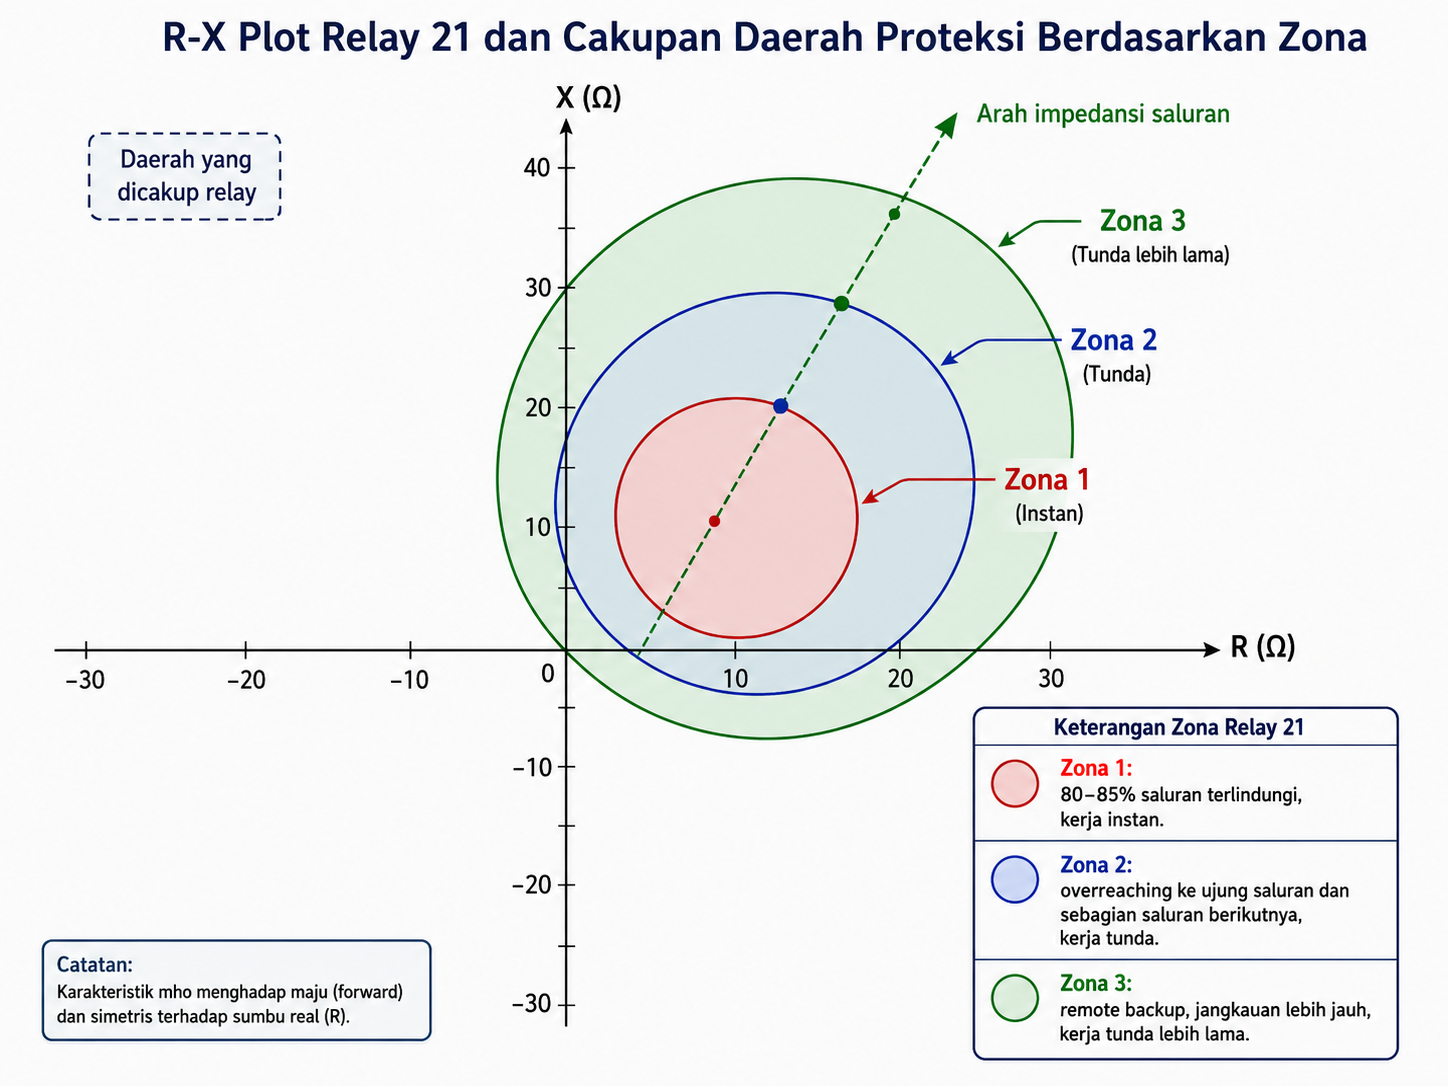
\includegraphics[width=0.9\textwidth]{contents/chapter-2/penjelasan zona 21.png}
    \caption{R-X plot of relay 21 and zone-based protection coverage}
    \label{fig:rx_plot_relay21_zona}
\end{figure}

The zone division of relay 21 can be illustrated on the R-X plane, as shown in Figure \ref{fig:rx_plot_relay21_zona}. On this plane, the R-axis represents the resistive component, while the X-axis represents the reactive component of the apparent impedance calculated by the relay. The \textit{mho} characteristic forms a protection region oriented in the direction of the line impedance. An apparent impedance point located within a zone characteristic can be identified as a fault within that zone's coverage. Zone 1 is used as instantaneous primary protection, while Zones 2 and 3 provide extended coverage with time delays for extended or backup protection. This division into several zones enables distance protection to maintain selectivity while providing backup coverage for subsequent lines \cite{abboud2019fivezones}.

Current sequence-component decomposition is used to transform the three-phase currents measured by the relay into zero-, positive-, and negative-sequence components. Given the phase-current phasors \(I_a\), \(I_b\), and \(I_c\), the decomposition can be expressed as follows:

\begin{equation}
    \begin{bmatrix}
        I_0 \\
        I_1 \\
        I_2
    \end{bmatrix}
    =
    \frac{1}{3}
    \begin{bmatrix}
        1 & 1 & 1       \\
        1 & a & a^2     \\
        1 & a^2 & a
    \end{bmatrix}
    \begin{bmatrix}
        I_a \\
        I_b \\
        I_c
    \end{bmatrix},
    \qquad a = 1\angle 120^\circ
    \label{eq:dekomposisi_urutan_arus}
\end{equation}

In Equation \ref{eq:dekomposisi_urutan_arus}, \(I_1\) represents the positive-sequence component, \(I_2\) represents the negative-sequence component, and \(I_0\) represents the zero-sequence component. The positive-sequence component corresponds to the balanced portion of the current that follows the normal phase sequence. The negative-sequence component appears when the three-phase currents are unbalanced, while the zero-sequence component corresponds to in-phase currents that commonly occur in faults involving ground or a neutral path. In the context of relay 21, this separation is important because unbalanced faults can alter the current composition used by the relay to derive the apparent impedance.

Liu \textit{et al.} identified the positive-, negative-, and zero-sequence voltages and currents measured by the relay as important quantities in the analysis of distance protection on IBR-connected lines during unbalanced faults. Their study also showed that reduced fault-current contribution in weak systems can cause \textit{underreach} or \textit{overreach} of the grid-side distance relay \cite{liu2025sequence}. Therefore, this research uses current sequence-component decomposition to determine whether the fault current entering relay 21 is dominated only by the positive-sequence component or also contains negative- and zero-sequence components.

For phase-to-ground elements, the zero-sequence component is important because the apparent impedance calculation of a \textit{ground distance} element requires zero-sequence compensation. Tsimtsios and Nikolaidis explained that the zero-sequence compensation factor \(K_0\) is a setting related to the positive- and zero-sequence impedances of the line and affects the operating accuracy of the \textit{ground distance} element during a single-line-to-ground fault \cite{tsimtsios2018setting}. Xu \textit{et al.} also used negative-sequence, zero-sequence, and combined negative-zero-sequence current components in a \textit{ground distance relaying} algorithm for high-resistance faults, indicating that sequence components can serve as additional indicators for interpreting phase-to-ground faults \cite{xu2010ground}.

This relationship becomes more important in systems with IBRs because fault current is not only limited in magnitude but can also be shaped by inverter control strategies. Liu \textit{et al.} showed that negative-sequence current injection from converter-based sources during faults can alter the converter fault response and introduce uncertainty into existing AC protection \cite{liu2025impact}. Xie \textit{et al.} also identified the compatibility of distance protection with various inverter control schemes as an issue requiring investigation. Therefore, \(I_1\), \(I_2\), and \(I_0\) should be considered when comparing relay 21 responses among different IBR types \cite{xie2025distance}.

In systems with IBRs, apparent impedance measurements may deviate because the fault current entering the relay is influenced by inverter controls. Hooshyar \textit{et al.} showed that lines connected to fully converter-interfaced renewable power plants may cause distance relays to fail to detect internal faults or to operate incorrectly for external faults \cite{hooshyar2015cirepp1}. Fang \textit{et al.} also demonstrated that \textit{inverter-interfaced renewable energy generators} can affect distance protection performance, indicating the need for enhanced schemes \cite{fang2019impact}.

In addition to limited current magnitude, the phase angle of the fault current may change because of inverter control strategies. This is important because distance relays depend not only on current magnitude but also on the phasor relationship between voltage and current. Sarkar \textit{et al.} emphasized that distance relay performance must be reassessed in future converter-dominated systems \cite{sarkar2017distance_relay_future}. Accordingly, the evaluation of relay 21 in this research examines whether settings based on a conventional system continue to produce appropriate operating characteristics when the type of IBR connected to the system changes.

\section{Operating Principle of Relay 87L}

Relay 87L, or the line current differential relay, operates by comparing the currents entering and leaving a transmission line. Under normal conditions or during external faults, the currents at the boundaries of the protection zone should ideally be balanced, resulting in a small differential current. During an internal fault, this balance is lost and the differential current increases. This principle makes 87L a fast and selective transmission line protection function, particularly when supported by communication between the line terminals \cite{ieee2015c37243}.

In practical implementations, relay 87L uses not only differential current but also \textit{restraint current}. Its operating characteristic is generally designed to maintain security against measurement errors, current-transformer (CT) mismatch, CT saturation, or external faults with large currents. Kasztenny \textit{et al.} explained that the characteristics of modern differential relays, including those used in multiterminal applications, depend on the relationship between the operating and restraint quantities \cite{kasztenny2011tutorial_multiterminal}.

In a two-terminal application, the operating quantity can be expressed as the differential current, while the restraint quantity can be derived from the average current magnitude at both ends of the line. Using \(I_A\) and \(I_B\) as the currents at the two line terminals, the differential current \(I_d\) and restraint current \(I_r\) can be expressed as follows \cite{thompson2010percentage}:

\begin{align}
    I_d & = \left| I_A + I_B \right| \label{eq:arus_diferensial_87l}                      \\
    I_r & = \frac{\left| I_A \right| + \left| I_B \right|}{2} \label{eq:arus_penahan_87l}
\end{align}

According to Equation \ref{eq:arus_diferensial_87l}, the differential current indicates the current imbalance entering the protection zone. Meanwhile, Equation \ref{eq:arus_penahan_87l} defines the restraint current used as a reference to prevent the relay from operating because of minor imbalances or external fault conditions.

\begin{figure}[H]
    \centering
    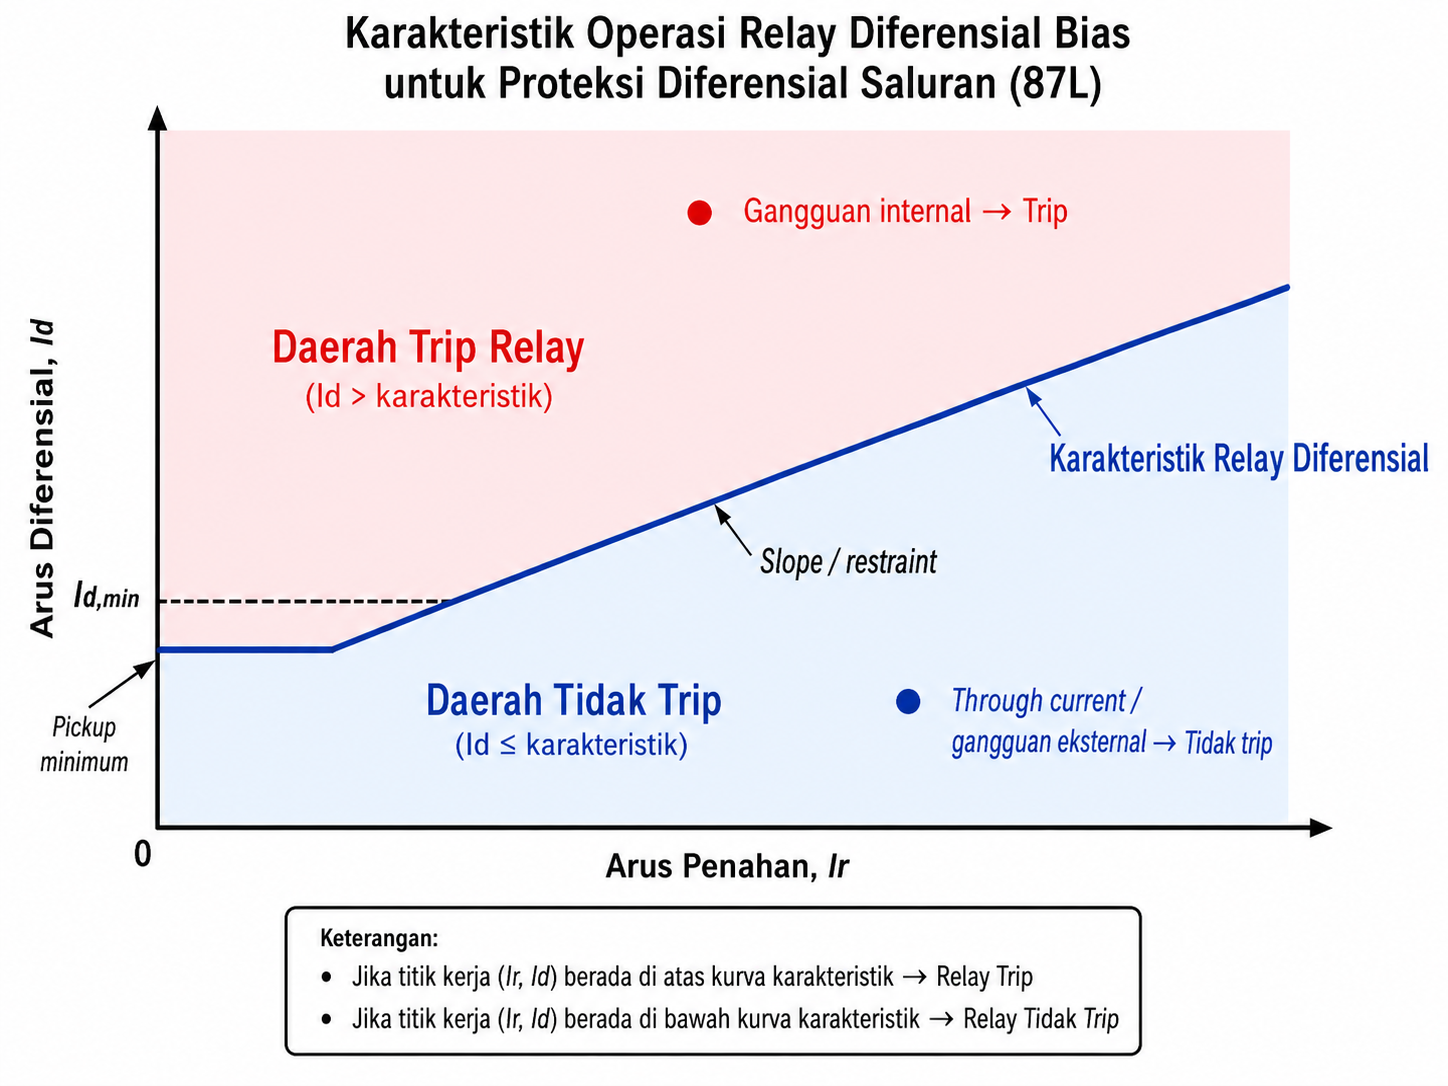
\includegraphics[width=0.85\textwidth]{contents/chapter-2/plot 87L.png}
    \caption{Operating characteristic of a line current differential relay}
    \label{fig:karakteristik_operasi_87l}
\end{figure}

The relationship between \(I_d\) and \(I_r\) can be represented by the biased differential relay operating characteristic shown in Figure \ref{fig:karakteristik_operasi_87l}. The characteristic curve separates the trip and no-trip regions. At low restraint current, the relay still requires a minimum differential current as its pickup threshold. Above this threshold, the operating limit increases according to the characteristic \textit{slope}. Thus, an operating point \((I_r, I_d)\) above the curve indicates relay operation, while a point below the curve indicates a restrained or no-trip condition. This biased characteristic allows the relay to remain sensitive to internal faults while maintaining security against \textit{through current}, external faults, measurement errors, and CT saturation \cite{anderson2017summary,thompson2010percentage,hedding2008line}.

In systems with IBRs, relay 87L faces challenges because the fault current at one or both ends of the line may be limited and controlled by inverters. Li \textit{et al.} found that inverter-based renewable generation can alter the characteristics of the currents used in line current differential protection calculations \cite{li2017analysis}. Consequently, the relationship between differential and restraint currents must be reassessed, particularly for internal faults, external faults, and changes in network configuration.

A subsequent study by Chowdhury, McDaniel, and Fischer stated that 87L elements in systems with IBRs may experience reduced \textit{dependability} and, if not properly applied, degraded \textit{security} \cite{chowdhury2023lcd}. This statement is relevant to the present research because 87L is not treated merely as a general solution; instead, its characteristics are examined while retaining settings based on a conventional system.

\section{Effects of IBRs on Transmission Protection Performance}

The effects of IBRs on transmission protection can be observed through changes in the electrical quantities used by the relays. For relay 21, the primary change concerns the apparent impedance estimate. Because apparent impedance is calculated from voltage and current, limited fault current, inverter-controlled current angles, and changes in contributions from the line terminals can shift the relay operating point away from its expected characteristic \cite{hooshyar2015cirepp1,fang2019impact,quispe2022transmission_review}.

For relay 87L, the effects of IBRs appear in the relationship between differential and restraint currents. During an internal fault, inverter-limited current may reduce the operating margin and potentially make the relay less sensitive. During an external fault or under certain network configurations, differences in the phase and dynamics of IBR currents may affect relay security if the settings do not account for the characteristics of inverter-based sources \cite{li2017analysis,chowdhury2023lcd}.

Chowdhury and Fischer placed this issue in a broader context. They stated that IBR responses during faults are inconsistent with those of synchronous sources and may therefore challenge the reliability of conventional transmission line protection schemes \cite{chowdhury2021tlp1}. In this research, that concept serves as the starting point, but the scope of the analysis is focused on two protection functions evaluated individually: relay 21 and relay 87L.

Modern interconnection standards also influence how IBRs respond to faults. IEEE Std 2800-2022 specifies the interconnection and interoperability capabilities of IBRs in transmission power systems, including performance expectations during faults and unbalanced voltage conditions \cite{ieee2022std2800}. Because IBR behavior during faults can be shaped by standards, manufacturer controls, and device settings, protection evaluations cannot rely solely on ideal-source assumptions such as those used in conventional system studies.

\section{Review of Previous Studies}

Chowdhury and Fischer conducted a key study on transmission line protection issues in systems with IBRs. Part I discussed protection problems arising from IBR responses during faults, while Part II discussed solutions and setting modifications that can improve protection reliability \cite{chowdhury2021tlp1,chowdhury2021tlp2}. These two papers form the primary basis of this research. However, the present research does not replicate the complete range of protection functions discussed in those papers and instead focuses its analysis on relay 21 and relay 87L.

Regarding relay 21, Hooshyar \textit{et al.} discussed distance protection problems on lines connected to fully converter-interfaced renewable power plants \cite{hooshyar2015cirepp1}. Their subsequent paper proposed and evaluated a solution to these problems \cite{hooshyar2015distance_part2}. Fang \textit{et al.} also demonstrated the effects of inverter-interfaced renewable energy generators on distance protection and proposed an improved scheme \cite{fang2019impact}. These studies indicate that relay 21 is a protection function sensitive to the characteristics of IBR sources.

Regarding relay 87L, Li \textit{et al.} analyzed line current differential protection in the presence of inverter-based renewable generation \cite{li2017analysis}. Chowdhury, McDaniel, and Fischer subsequently discussed the challenges and solutions associated with applying 87L in systems with IBRs \cite{chowdhury2023lcd}. These two studies establish that relay 87L, although often considered highly selective, still requires investigation in systems containing inverter-controlled fault-current sources.

A review by Quispe \textit{et al.} showed that the principal transmission line protection challenges in systems with IBRs are related to changes in current magnitude, phase angle, negative-sequence components, and short-circuit current levels \cite{quispe2022transmission_review}. Meanwhile, Haddadi \textit{et al.} discussed the effects of IBRs on power system protection in general, including elements that use negative-sequence quantities \cite{haddadi2021systemprotection,haddadi2021negative_sequence_elements}. This literature reinforces the need to evaluate transmission protection when IBRs are introduced into systems whose protection settings still follow conventional assumptions.

A summary of the literature used in this chapter is presented in Table \ref{tab:matriks_literatur_posisi}. The table serves not only as a literature summary but also as a basis for establishing the position of this research. Each reference is therefore categorized according to its research focus, approach, principal contribution, and relevance to the evaluation of relay 21 and relay 87L in transmission systems with IBR integration.

\begingroup
% Avoid infinite-shrink warnings when longtable splits across pages.
\let\vss\vfil
% Suppress expected underfull-box diagnostics in narrow table columns.
\hbadness=10000
\scriptsize
\setlength{\LTleft}{0pt}
\setlength{\LTright}{\fill}
\setlength{\tabcolsep}{2pt}
\renewcommand{\arraystretch}{1.22}
\newcommand{\thead}[1]{\makebox[\linewidth][c]{\shortstack{#1}}}
\begin{longtable}{|p{0.14\textwidth}|p{0.10\textwidth}|p{0.16\textwidth}|p{0.15\textwidth}|p{0.18\textwidth}|p{0.20\textwidth}|}
    \caption{Literature Matrix Establishing the Research Position}
    \label{tab:matriks_literatur_posisi} \\
    \hline
    \thead{\textbf{Author/}\\\textbf{Year}} &
    \thead{\textbf{Literature}\\\textbf{Type}} &
    \thead{\textbf{Research}\\\textbf{Focus}} &
    \thead{\textbf{Method/}\\\textbf{Approach}} &
    \thead{\textbf{Principal}\\\textbf{Contribution}} &
    \thead{\textbf{Relevance to}\\\textbf{This Research}} \\ \hline
    \endfirsthead

    \caption[]{Literature Matrix Establishing the Research Position (continued)} \\
    \hline
    \thead{\textbf{Author/}\\\textbf{Year}} &
    \thead{\textbf{Literature}\\\textbf{Type}} &
    \thead{\textbf{Research}\\\textbf{Focus}} &
    \thead{\textbf{Method/}\\\textbf{Approach}} &
    \thead{\textbf{Principal}\\\textbf{Contribution}} &
    \thead{\textbf{Relevance to}\\\textbf{This Research}} \\ \hline
    \endhead

    Nimpitiwan \textit{et al.} (2007) \cite{nimpitiwan2007fault_current_contribution} & Journal article & Fault-current contributions from synchronous machines and inverter-based generators & Fault-current contribution analysis & Demonstrates differences in fault-current characteristics between conventional and inverter-based sources & Provides a basis for comparing fault-current contributions from conventional systems and IBRs \\ \hline

    IEEE/NERC Task Force (2018) \cite{ieeenerc2018tr68} & Technical report & Effects of inverter-based generation on system dynamics and short-circuit performance & Technical power-system study & Explains that IBRs can alter power-system short-circuit performance & Supports the need to evaluate protection when short-circuit current levels and characteristics change \\ \hline

    Haddadi \textit{et al.} (2021) \cite{haddadi2021systemprotection} & Journal article & Effects of IBRs on power-system protection & Study of IBR effects on protection elements & Summarizes the effects of IBRs on power-system protection functions & Establishes the general basis for reassessing protection settings when IBR sources are integrated into the grid \\ \hline

    IEEE Std 2800 (2022) \cite{ieee2022std2800} & Standard & Interconnection and interoperability of IBRs in transmission power systems & Technical interconnection standard & Specifies performance requirements for IBRs connected to transmission systems & Establishes that IBR behavior during faults is influenced by interconnection requirements and device controls \\ \hline

    Chowdhury and Fischer (2021a) \cite{chowdhury2021tlp1} & Journal article & Transmission line protection problems in systems with IBRs & Analysis and testing of protection schemes & Identifies transmission line protection problems caused by IBR responses during faults & Provides the primary problem framework, with the scope narrowed to relay 21 and relay 87L \\ \hline

    Nagpal \textit{et al.} (2020) \cite{nagpal2020tr81} & Technical report & Protection challenges and practices for IBR interconnection in transmission systems & Protection committee technical report & Summarizes protection challenges when IBRs are connected to utility transmission systems & Reinforces the need to reassess transmission protection in systems with IBRs \\ \hline

    Quispe \textit{et al.} (2022) \cite{quispe2022transmission_review} & Review article & IBR-related transmission line protection challenges & Literature review & Maps the effects of IBRs on current magnitude, phase angle, sequence components, and short-circuit levels & Provides the basis for selecting evaluation indicators such as fault current, apparent impedance, and relay response \\ \hline

    English \textit{et al.} (2011) \cite{english2011current_contributions} & Conference paper & Fault-current contributions from Type 3 and Type 4 wind turbines & Analysis of current contributions during faults & Shows that Type 3 and Type 4 wind-turbine current contributions differ from synchronous-machine assumptions & Supports the selection of Type 3 and Type 4 wind turbines as the IBR types being compared \\ \hline

    Kou \textit{et al.} (2020a) \cite{kou2020fault} & Journal article & Fault characteristics of solar power plants & Analysis of PV fault-current characteristics & Shows that the PV fault-current contribution is shaped by inverter controls & Provides the basis for considering PV as one of the IBR types tested in this research \\ \hline

    Kou \textit{et al.} (2020b) \cite{kou2020negative_sequence} & Journal article & Negative-sequence current injection from transmission-connected solar power plants & Negative-sequence component analysis & Highlights concerns regarding negative-sequence injection from solar power plants & Supports the discussion that sequence quantities and fault direction can affect protection elements \\ \hline

    Haddadi \textit{et al.} (2021) \cite{haddadi2021negative_sequence_elements} & Journal article & Effects of IBRs on negative-sequence-based protection elements & Protection-element analysis & Explains the effects of IBRs on negative-sequence quantities used by protection systems & Supports protection evaluation when fault currents and sequence components are influenced by inverter controls \\ \hline

    IEEE Std C37.113 (2016) \cite{ieee2016c37113} & Standard & Application of protective relays on transmission lines & Transmission line protection application guide & Explains the application principles of transmission line protective relays & Provides the theoretical basis for relay 21 and distance protection zoning principles \\ \hline

    Schweitzer and Roberts (2010) \cite{schweitzer2010distance_relay_element_design} & Technical article & Distance relay element design & Technical explanation of relay elements & Explains the calculation and design concepts of distance relay elements & Provides the basis for understanding the apparent impedance used by relay 21 \\ \hline

    Abboud \textit{et al.} (2019) \cite{abboud2019fivezones} & Conference paper & Use of multiple zones in distance protection & Technical study of protection-zone applications & Explains the benefits of dividing distance protection into zones & Supports the explanation of relay 21 zone characteristics on the R-X plane \\ \hline

    Tsimtsios and Nikolaidis (2018) \cite{tsimtsios2018setting} & Journal article & Zero-sequence compensation factor in distance relays & Theoretical analysis and setting study & Explains that \(K_0\) affects the accuracy of the \textit{ground distance} element during single-line-to-ground faults & Provides the basis for discussing zero-sequence components and compensation in relay 21 \\ \hline

    Xu \textit{et al.} (2010) \cite{xu2010ground} & Journal article & \textit{Ground distance} algorithm for high-resistance faults & Use of negative-sequence, zero-sequence, and combined negative-zero-sequence current components & Uses current sequence components to estimate phase-to-ground fault impedance & Supports the interpretation of sequence components when assessing phase-to-ground faults using relay 21 \\ \hline

    Hooshyar \textit{et al.} (2015a) \cite{hooshyar2015cirepp1} & Journal article & Distance protection on lines connected to fully converter-interfaced power plants & Problem statement and protection analysis & Demonstrates the potential failure or misoperation of distance relays in converter-based systems & Establishes that relay 21 is sensitive to IBR fault-current characteristics \\ \hline

    Fang \textit{et al.} (2019) \cite{fang2019impact} & Journal article & Effects of inverter-based renewable generation on distance protection & Impact analysis and proposed improved scheme & Demonstrates changes in distance relay performance caused by inverter-based sources & Supports the evaluation of apparent impedance changes and relay 21 operating decisions \\ \hline

    Sarkar \textit{et al.} (2017) \cite{sarkar2017distance_relay_future} & Conference paper & Distance relay performance in converter-dominated systems & Relay performance analysis & Demonstrates the need to evaluate distance relays in future converter-based systems & Reinforces the importance of analyzing relay 21 in systems with IBRs \\ \hline

    Liu \textit{et al.} (2025a) \cite{liu2025sequence} & Journal article & Sequence-component-based distance protection for IBR-connected lines during unbalanced faults & Sequence-component algorithm and RTDS simulation & Demonstrates \textit{underreach} and \textit{overreach} issues and the use of local sequence quantities in distance relays & Provides the basis for discussing current sequence-component decomposition for relay 21 \\ \hline

    Liu \textit{et al.} (2025b) \cite{liu2025impact} & Conference paper & Effects of converter negative-sequence current injection on distance protection & Analysis and \textit{hardware-in-the-loop} testing & Demonstrates that negative-sequence current injection can alter converter fault responses and create risks for AC protection & Supports the need to examine negative-sequence components in systems with IBRs \\ \hline

    Xie \textit{et al.} (2025) \cite{xie2025distance} & Journal article & Distance protection for IBR-connected lines under various inverter control schemes & Study of distance protection under different inverter controls & Identifies the compatibility of distance protection with various inverter control schemes as an issue requiring investigation & Supports the use of sequence-component decomposition when comparing relay 21 responses among different IBR types \\ \hline

    IEEE Std C37.243 (2015) \cite{ieee2015c37243} & Standard & Application of digital line current differential relays & Relay 87L application guide & Explains the use of line current differential relays based on digital communication & Provides the theoretical and modeling basis for relay 87L on line TL89 \\ \hline

    Kasztenny \textit{et al.} (2011) \cite{kasztenny2011tutorial_multiterminal} & Tutorial paper & Operating characteristics of multiterminal line current differential relays & Technical tutorial on differential relays & Explains the operating characteristics of microprocessor-based differential relays & Provides the basis for interpreting the operating and restraint regions of relay 87L \\ \hline

    Thompson (2010) \cite{thompson2010percentage} & Conference paper & \textit{Percentage restrained differential} principle & Technical explanation of differential calculations & Explains the meaning of differential and restraint currents in differential relays & Provides the basis for the equations and interpretation of the relationship between \(I_d\) and \(I_r\) \\ \hline

    Anderson (2017) \cite{anderson2017summary} & Technical report & Summary of the IEEE C37.243 guide for digital differential relays & Technical summary of the standard & Summarizes applications of digital line current differential relays & Supports the explanation of relay 87L operating characteristics \\ \hline

    Hedding and Holst (2008) \cite{hedding2008line} & Conference paper & Differential relay operation during severe CT saturation & Analysis of relay operating conditions & Demonstrates the importance of differential relay security under nonideal measurement conditions & Establishes that relay 87L must account for restraint current and operating security \\ \hline

    Li \textit{et al.} (2017) \cite{li2017analysis} & Conference paper & Line current differential protection with inverter-based renewable generation & Analysis of inverter-source effects on 87L & Shows that inverters can alter the currents used in differential relay calculations & Provides the basis for evaluating relay 87L in systems with IBRs \\ \hline

    Chowdhury \textit{et al.} (2023) \cite{chowdhury2023lcd} & Conference paper & Challenges and solutions for relay 87L in systems with IBRs & Study of differential protection challenges and solutions & Explains \textit{dependability} and \textit{security} issues affecting relay 87L in systems with IBRs & Supports the conclusion that relay 87L still requires evaluation despite its selectivity \\ \hline

    Chowdhury and Fischer (2021b) \cite{chowdhury2021tlp2} & Journal article & Transmission line protection solutions for systems with IBRs & Evaluation of solutions and setting modifications & Proposes approaches to improve transmission line protection reliability in systems with IBRs & Provides a comparison showing that this research focuses on evaluating relay responses rather than optimizing new settings \\ \hline

    Hooshyar \textit{et al.} (2015b) \cite{hooshyar2015distance_part2} & Journal article & Distance protection solution for lines connected to fully converter-interfaced power plants & Description and evaluation of the solution & Evaluates an improved approach to distance protection problems in converter-based systems & Provides a comparison with the scope of this research, which assesses the suitability of conventional settings \\ \hline
\end{longtable}
\endgroup

\section{Research Position and Contributions}

Based on the literature review, this research is positioned as a focused replication study of the problem framework proposed by Chowdhury and Fischer \cite{chowdhury2021tlp1}. This replication does not repeat the complete scope of their paper; instead, it reexamines the central idea within a narrower scope, namely the characteristics of relay 21 and relay 87L in transmission systems with IBRs.

The first contribution of this research is a comparison of two transmission line protection functions with different operating principles. Relay 21 is analyzed through changes in apparent impedance and operating decisions, while relay 87L is analyzed through changes in differential current, restraint current, and operating decisions. This comparison is important because IBRs can affect the two relays through different mechanisms.

The second contribution is the use of three IBR types as the primary variable: Type 3 wind turbines, Type 4 wind turbines, and photovoltaic systems. The IBR penetration level is kept constant so that differences in the results can be more directly associated with the characteristics of each IBR technology. The third contribution is the evaluation of several fault-location scenarios and a condition in which one transmission line is \textit{out of service}, ensuring that the analysis is not limited to a single network condition.

With this research position, the results are expected to provide a basis for determining the applicability limits of conventional settings, the need for setting adjustments, and the potential implementation of supplementary protection approaches in transmission systems with IBRs.
